\documentclass[11pt,a4paper,twocolumn]{article}
\usepackage[T1]{fontenc}
\usepackage[utf8]{inputenc}
\usepackage{anysize, longtable}
\usepackage{amsthm, amsfonts, amsmath, amssymb, booktabs, float}
\usepackage{sectsty, csquotes, xcolor, xspace, setspace, listings}
\usepackage{graphicx, tabularx, changepage, multirow, subcaption}
\usepackage{algorithm, algpseudocode, multicol, cuted, colortbl}
\usepackage{makecell, supertabular, stfloats}
\usepackage[hidelinks,bookmarksdepth=3]{hyperref}
\usepackage[capitalise]{cleveref}
\usepackage[inline]{enumitem}
\usepackage[english]{babel}
\usepackage{microtype}
\usepackage{libertinus}
\usepackage[scale = 0.85]{plex-mono}
\usepackage[maxbibnames=99]{biblatex}
\usepackage{titlesec}
\usepackage{tikz}

\usetikzlibrary{fit, shapes.geometric, positioning, shapes.misc, calc, arrows.meta, patterns, backgrounds, decorations, decorations.markings, decorations.pathreplacing, shadows, hobby}

\makeatletter

\thispagestyle{empty}

\theoremstyle{plain}
\newtheorem{theorem}{Theorem}
\newtheorem{lemma}{Lemma}

\theoremstyle{definition}
\newtheorem{definition}{Definition}
\newtheorem{example}{Example}

\theoremstyle{remark}
\newtheorem*{note}{Note}
\newtheorem*{remark}{Remark}

\newcommand{\inlinecode}[1]{\lstinline[basicstyle=\ttfamily,columns=fixed]$#1$}
\lstset{basicstyle=\setstretch{0}\small\ttfamily,breaklines=true,columns=fixed,captionpos=b,xleftmargin=0.5cm}

\newlength{\offsetpage}
\newenvironment{widepage}[1][2cm]{
  \setlength{\offsetpage}{#1}
  \begin{adjustwidth}{-\offsetpage}{-\offsetpage}
  \addtolength{\linewidth}{2\offsetpage}
}{\end{adjustwidth}}

\algnewcommand{\IIf}[1]{\State \algorithmicif\ #1\ \algorithmicthen}
\algnewcommand{\IElse}[1]{\algorithmicelse\ #1}
\algnewcommand{\EndIIf}{\unskip\ \algorithmicend\ \algorithmicif}

\addbibresource{biblio.bib}

\allowdisplaybreaks
\marginsize{2.0cm}{2.0cm}{1.25cm}{1.25cm}
\setcounter{tocdepth}{2}
\setlist[itemize]{topsep=0pt, partopsep=0pt, parsep=0pt, itemsep=\parskip}
\setlist[enumerate]{topsep=0pt, partopsep=0pt, parsep=0pt, itemsep=\parskip}
\titlespacing*{\section}{0pt}{0.5\baselineskip}{0.1\baselineskip}
\titlespacing*{\subsection}{0pt}{0.4\baselineskip}{0.1\baselineskip}
\titlespacing*{\subsubsection}{0pt}{0.3\baselineskip}{0.1\baselineskip}
\titlespacing*{\paragraph}{0pt}{0pt}{0.5\baselineskip}
\hbadness=10000

\title{Assessing Infrastructure Vulnerability to \\Natural Hazards in South Tyrol}
\author{Roland Bernard, 19598, \inlinecode{rolbernard@unibz.it}}
\date{December 2025}

\def\maketitle{
\begin{strip}
  \begin{adjustwidth}{5mm}{5mm}
    \vspace{-4.5em}
    \noindent{\small\bfseries Project Proposal -- Data Curation 2025/2026\par}
    \vskip 0.25em
    \noindent{\LARGE\bfseries \@title\par}
    \vskip 1em
    \noindent{\large \@author\par}
    \vskip 1em
    \noindent{\small \@date\par}
    \vskip 1em
  \end{adjustwidth}
\end{strip}
}
\renewenvironment{abstract}{
  \vskip 1em
  \begin{quote}
  {\normalsize \abstractname\par}
  \small
}{
  \end{quote}
  \vskip 1em
}

\makeatother

\begin{document}

\maketitle

\begin{figure*}[b!]
  \centering
  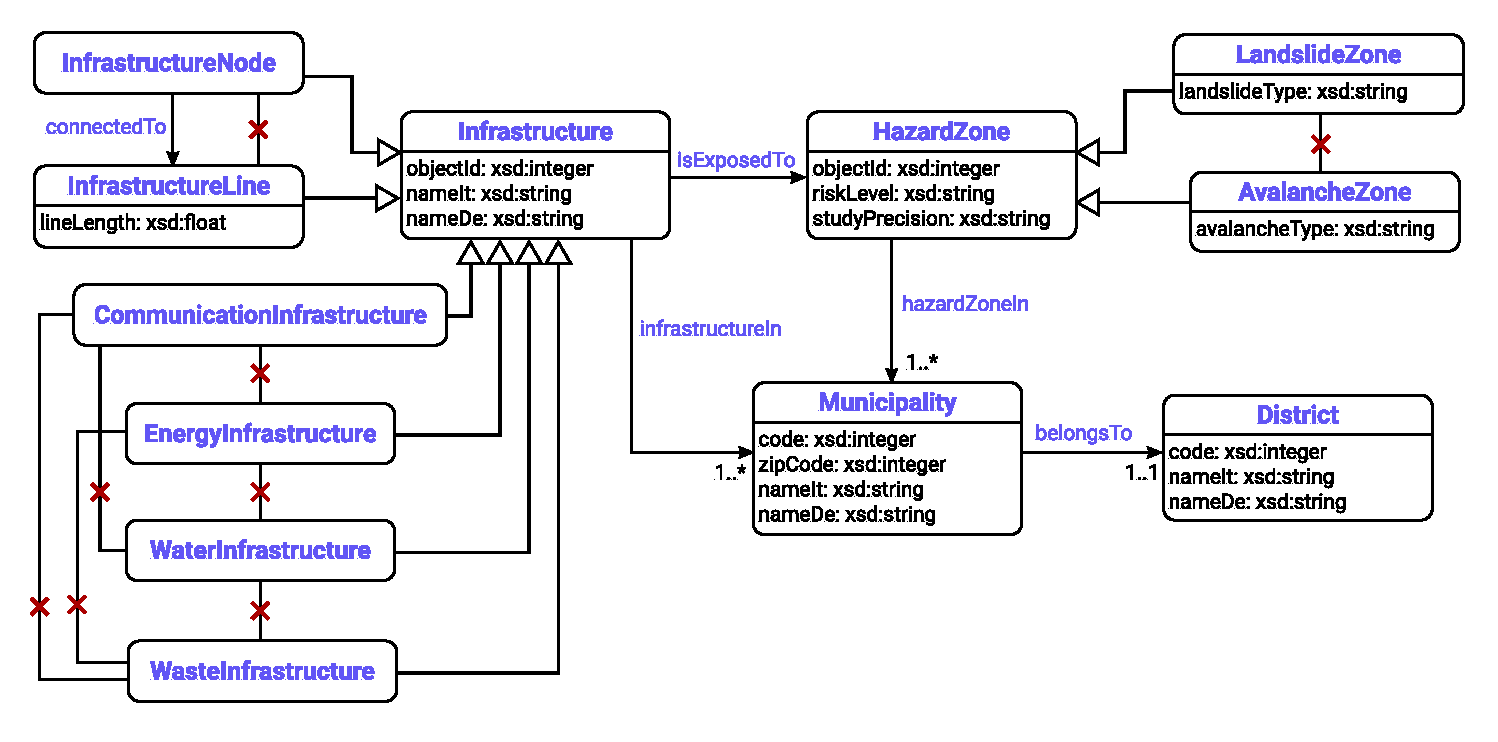
\includegraphics[width=\linewidth]{figures/ontology.pdf}
  \caption{Proposed ontology for the project.}
  \label{fig:ontology}
\end{figure*}

\section{Domain of Interest} \label{domain}

The idea of the project is to focus on the intersection of exposed assets and natural hazards. The aim is to identify and analyze critical infrastructure (water, electricity, and communications) that are geographically located within known hazard zones (landslides and avalanches) to assess potential vulnerabilities.

\section{Data Sources} \label{datasources}

The project will integrate five datasets from the Bolzano Province GeoKatalog. The integration will involve the following provided data sources:
\begin{itemize}
  \item \textbf{Infrastructure:} \inlinecode{bz_infrastructure_line} and \inlinecode{bz_infrastructure_node} for providing information about critical infrastructure.
  \item \textbf{Hazards:} \inlinecode{bz_hazard_landslide} and \inlinecode{bz_hazard_avalanche} provide information about know hazard zones.
  \item \textbf{Administrative:} \inlinecode{bz_admin_municipality} to provide spatial context and assign risk to specific municipalities.
\end{itemize}

\section{Application and Queries} \label{application}

By integrating infrastructure assets with hazard inventories and administrative data, the system will be able to answer the following types of queries:
\begin{itemize}
  \item Which water-related infrastructure nodes are located within high risk landslide zones?
  \item What are the infrastructure lines that intersect with avalanche-prone areas?
  \item In a given Municipality, how many electricity lines are currently situated in a hazard zone.
  \item Which municipalities have the highest count of infrastructure elements exposed to natural hazards?
\end{itemize}

\section{Initial Ontology} \label{technology}

An OWL 2 QL ontology with will be created that contains relevant classes (e.g., Infrastructure, HazardZone, Municipality, PowerLine) and properties (e.g., isLocatedIn, intersectsHazard). A preliminary design for the ontology is shown in \cref{fig:ontology}.

\end{document}
